\documentclass[article]{jss}
\usepackage[utf8]{inputenc}

\providecommand{\tightlist}{%
  \setlength{\itemsep}{0pt}\setlength{\parskip}{0pt}}

\author{
WenjingWang\\Renmin University of China \And Dianne Cook\\Monash University \And Earo Wang\\Monash University
}
\title{}

\Plainauthor{WenjingWang, Dianne Cook, Earo Wang}
\Plaintitle{Diagnosing Outliers and Visualization of Quantile Regression Models}

\Abstract{
Quantile regression models have been widely used in numerous
applications, and the subject of substantial research. In a recent
review article (\citet{koenker2017}) that surveys the research in the
for the past 40 years, one recommendation is that more diagnostics
should be provided for modeling. Estimation has been the priority, but
diagnosing the models is lacking. This paper provides diagnostics for
assessing the robustness of quantile regression models and implements
outlier detection methods in the R (\citet{RCore}) package
\texttt{quokar}. The package contains functions and plots for detecting
outliers in quantile regression.
}

\Keywords{Outlier diagnostic, Quantile regression, Robust distance, Generalized Cook's distance, Q-function distance, Bayes}
\Plainkeywords{Outlier diagnostic, Quantile regression, Robust distance, Generalized Cook's distance, Q-function distance, Bayes}

%% publication information
%% \Volume{50}
%% \Issue{9}
%% \Month{June}
%% \Year{2012}
%% \Submitdate{}
%% \Acceptdate{2012-06-04}

\Address{
    WenjingWang\\
  Renmin University of China\\
  Department of Statistics, Renmin University of China, China 100872\\
  
  
      Dianne Cook\\
  Monash University\\
  Department of Econometrics and Business Statistics, Monash University,
  VIC 3800 Australia\\
  
  
      Earo Wang\\
  Monash University\\
  Department of Econometrics and Business Statistics, Monash University,
  VIC 3800 Australia\\
  
  
  }

\usepackage{amsmath} \usepackage{amsfonts}

\usepackage{amsthm}
\newtheorem{theorem}{Theorem}[section]
\newtheorem{lemma}{Lemma}[section]
\theoremstyle{definition}
\newtheorem{definition}{Definition}[section]
\newtheorem{corollary}{Corollary}[section]
\newtheorem{proposition}{Proposition}[section]
\theoremstyle{definition}
\newtheorem{example}{Example}[section]
\theoremstyle{remark}
\newtheorem*{remark}{Remark}
\begin{document}

\section{Introduction}\label{introduction}

\subsection{Where QR is used}\label{where-qr-is-used}

Quantile regression model has been widely used in many research areas
such as economy, finance and social science (see
\citet{autor2017effect}, \citet{mitchell2017physical},
\citet{gallego2017corporate}, \citet{maciejowska2016probabilistic}).
Quantile regression provides improvements on mean regression because,
(a) observed covariates can describe the full distribution of a response
variable, and (b) estimators can maintain optimal properties in the
presence of heteroscedasticity or heavy tailed distributions.

\subsection{Types of QR algorithms}\label{types-of-qr-algorithms}

The research scope of quantile regression has been broadened
considerably in the past decades. We surveyed some of the most recent
developments: \citet{koenker2004quantile}, \citet{geraci2006use}
conducted quantile regression for longitudinal data. Longitudinal data
introduced a large number of ``fixed effects'' in quantile regression
and these ``fixed effects'' will significantly inflate the variability
of estimates of other covariate effects. They proposed to use \(l^1\)
regularization methods as essential computational tools.
\citet{parente2016quantile} studied properties of the quantile
regression estimator when data are sampled from independent and
identically distributed clusters. They provided a consistent estimator
of the covaiance matrix and showed the regression estimator is
consistent and asympototically normal. Researchers
(\citet{galvao2011quantile}, \citet{canay2011simple}) also construct
quantile regression model using panel data. Panel data potentially
integrate fixed effects to control unobserved covariates which extend
the original quantile regression model. They presented new model format
and fixed effects estimation.

Due to the advantages of quantile regression model possesed, researches
also interested in ebbeding it in other models to enhance model features
or conduct better results analysis. \citet{geraci2014linear} proposed
linear quantile mixed model which dealt with within-subject dependence
by embeding subject-specific random intercepts into quantile regression
model. Estimation strategies to reduce the computational burden and
inefficiency using EM algorithm. \citet{chernozhukov2006instrumental}
proposed instrumental variable quantile regression to evaluate the
impact of endogenous variables or treatments on the entire distribution
of outcomes. They modifies the conventional quantile regression and
recovers quantile-specific covariate effects in an instrumental
variables model.

\subsection{Inference}\label{inference}

Along with the continous progresses in model improvement and
application, extensive model inferencing research has been done.
\citet{gutenbrunner1993tests} proposed rank-based inference to deal
problems of constructing confidence intervals for individual quantile
regression parameter estimates. In order to quantify the robustness of
inferencing, resampling methods are studied at the same time
(\citet{hahn1995bootstrapping}, \citet{buchinsky1995estimating},
\citet{feng2011wild}). \citet{koenker1999goodness} used
Kolmogorov-Smironov method to measure the goodness of fit of quantile
regression. To tackle the ``Durbin problem'',
\citet{koenker2002inference} developed location shift and location-scale
shift test for quantile regression model. The inferencing study also
have been extended to Bayesian framework (\citet{yu2001bayesian},
\citet{yu2007bayesian}, \citet{kozumi2011gibbs},
\citet{santos2016bayesian}).

\subsection{Software}\label{software}

Effective toolboxes conduct fitting and inferencing for quantile
regression model has been developed based on the theoretical researches
mentioned above. Free software R offers several packages implementing
quantile regression, most famous \texttt{quantreg} by Roger Koenker, but
also \texttt{gbm}, \texttt{quantregForest}, \texttt{qrnn},
\texttt{ALDqr} and \texttt{bayesQR}. However, few diagnostic methods
were proposed for quantile regression and no toolbox for model
diagnostic were implemented in R. \citet{gu2017unobserved} pointed out
more work needs to be done to develop better diagnostic tools.

\subsection{Outlier diagnostics
generally}\label{outlier-diagnostics-generally}

Outlier detection is one important aspect of model diagnostic. It is
unignorable in regression analysis because the results of regression can
be sensitive to outliers. Data used for fitting regression model may
contain special points located far away from others either in response
variable or in the space of the predictors. The latter are also called
leverage points. In univariate model, outliers can be easily observed by
scatter plot of predictor and responsor. Difficulty lies in
high-dimensional situation, where statistical methods should be used.
Various methods for detecting outliers have been explored
(\citet{rousseeuw1990unmasking}, \citet{gather1997convergence}).
Commonly used statistics include residuals, leverage value, studentized
residuals and jacknife residuals.

In regression context, classic least ordinary square estimation of
linear regresssion can be expressed as
\(\hat{\boldsymbol{\beta}}=\boldsymbol{(X^{'}X)^{-1}X^{'}Y}\),
\(\hat{\boldsymbol{Y}}=\boldsymbol{X(X^{'}X)^{-1}X^{'}Y}=\boldsymbol{HY}\).
where, \(\boldsymbol{H}\) is called hat matrix. Residuals can be written
as
\(\hat{\boldsymbol{\epsilon}}=\boldsymbol{Y-\hat{Y}(1-H)Y}=\boldsymbol{(1-H)\epsilon}\).
Hence, if consider the influence of outliers in vertical direction and
leverage points at the same time, we should use studentized residuals,
which is \(r_i=\frac{\hat{\epsilon}_{i}}{\sigma^{2}\sqrt{1-h_i}}\). The
larger \(r_i\), the more suspicious the outlier is. Another widely used
outlier diagnositc framework is leave one out. Jackknife residual and
Cook's distance are constructed based on this idea. These diagnostic
statistics has already become available on widely distributed
statistical software packages SAS, SPSS, as well as R.

Estimating process of quantile regression differs from mean regression
which results no explicit solution form
\(\hat{\boldsymbol{\beta}}=\boldsymbol{(X^{'}X)^{-1}X^{'}Y}\). In
addition, quantile regressions can be fitted on any quantile interested
, which add difficulties in applying diagnosing methods and displaying
results simutaneously. \citet{sanchez2013likelihood} developed
case-deletion diagnostics for quantile regression using the asymmetric
Laplace distribution. \citet{santos2016bayesian} discussed Bayesian
quantile regression and considered using the posterior distribution of
the latent variable for outlier diagnosing. Toolbox for outlier
diagnostic can only be found in statistical software SAS in procedure
\texttt{QUANTREG}. To the authors' knowledge, these methods are still
not be implemented in R. In order to fill the gap, related
implementation in R language now is available in rencently developed
package \texttt{quokar} which provides several outlier diagnostic
methods as well as supportive visualization results for quantile
regression.

\subsection{Visualization for QR is
lacking}\label{visualization-for-qr-is-lacking}

Visualizations of high-dimensional data are well developed and explored.
Model visualizations are recently been studied.
\citet{wickham2015visualizing} first proposed the idea of plotting model
in data space. He pointed out that visual model can anwser questions
such as what does the model look like? how well does the model fit the
data? how does the shape of the model compare to the shape of the data?
is the model fitting uniformly good, or good in some regions but poor in
other regions. Integrating model and original data in one plot is a
straight-forward way to observe outliers for fitted model. To visualize
data and models in high dimensions, we need good tools:

\begin{itemize}
\item
  The grand tour. The grand tour generating a sequence of 2d projections
  of an p-d object. It randomly chooses new projections and rotates
  between them. Through this process, we can observe the distribution of
  data (clusted or sparse) and identify outliers.
\item
  Brushing. We use a brush to colour observations and models in one
  plot. In our case, regression models on different quantiles are
  brushed.
\end{itemize}

In this paper, we propose a general framework of quantile regression
visualization with \texttt{GGobi}. Linear quantile regression model in
3D and 4D data space and non-linear models are displayed as examples.

This article aims to introduce R package \texttt{quokar} and propose
general framework of visualizing quantile regression models in high
dimensional space. The remainder of this article is organized as
follows: In Section 2, we provide a general introduction to quantile
regression model and explore its robusness. In Section 3 we give a tour
of outlier diagnostic methods used in package \texttt{quokar}. In
section 4 we illustrate the usefulness of the package through a real
data set example. In section 5, we provide the geralize framework of
visualizing quantile regression. The summary and future research
directions are discussed in Section 6.

\section{Robustness of Quantile
Regression}\label{robustness-of-quantile-regression}

\citet{koenker1978regression} first proposed linear model as

\begin{equation}
y_i=x^{'}_{i}\beta_{\tau}+\epsilon_{i}, \quad i=1,...,n
\label{eq:linear_qr}
\end{equation}

The \(\tau\)th quantile function of the sample is
\(Q_{y}(\tau|x)=x^{'}\beta(\tau)\). Based on the idea of minimizing a
sum of asymmetrically weighted absolute residuals, the objective
function of quantile regression model is,

\begin{equation}
\min_{\beta_{\tau} \in \mathbb{R}^{p}}\sum_{i=1}^{n} \rho_{\tau}(y_i-x_{i}^{'}\beta_{\tau})
\label{eq:object_function}
\end{equation}

where \(\rho(.)\) is loss function which was defined as
\(\rho_{\tau}(u)=u(\tau-I(u <0))\). In addition, assuming
\(Y_1,...,Y_n\) is a sequence of i.i.d random variables which has
distribution function \(F\) and continuous density function \(f\). The
coefficience vector \(\hat{\boldsymbol{\beta}}_{\tau}\) is
asymptotically normal, which can be expressed as,

\begin{equation}
\sqrt{n}(\hat{\boldsymbol{\beta}}_{\tau}-\boldsymbol{\beta}_{\tau}) \xrightarrow{d}
N(0,\tau(1-\tau)\boldsymbol{D}\boldsymbol{\varOmega}_{x}\boldsymbol{D}^{-1})
\label{eq:distrbution}
\end{equation}

where
\(\boldsymbol{D}=E(f(\boldsymbol{X}\boldsymbol{\beta})\boldsymbol{X}\boldsymbol{X}^{'})\)
and \(\boldsymbol{\varOmega}_{x}=E(\boldsymbol{X}^{'}\boldsymbol{X})\).

Quantile is more robust than mean when extreme values exist in the
dataset interested. This property applies equally in regression context.
The robustness of quantile and quantile regression can be expressed by
influence function. \(F\) is distribution function of interested
variable. Set \(T\) as a function of \(F\), the influence function is
the directional derivative of \(T(F)\) at \(F\), and it measures the
effect of a small perturbation in \(F\) on \(T(F)\). For Mean, the
influence function is

\begin{equation}
IF(y;T;F)=y-T(F)
\label{eq:mean-influence}
\end{equation}

For the \(\tau\)th quantile points, influence function can be expressed
as,

\begin{equation}
IF(y;T;F)=\left\{
\begin{aligned}
\frac{\tau}{f(F^{-1}(\tau))} & ; & y > F^{-1}(\tau) \\
\frac{(\tau-1)}{f(F^{-1}(\tau))} & ; & y \leq F^{-1}(\tau) 
\end{aligned}
\right.
\label{eq:quantile-influence}
\end{equation}

where \(f\) is the density function of \(F\). Comparing
\eqref{eq:mean-influence} and \eqref{eq:quantile-influence}, the latter is a
bounded function with \(y\) changing in its domain. Figure
\ref{fig:vis-if} is an example plot of influence funtion. Data are
generated from distribution function \(F(x)=1-e^{-\lambda x},x>0\), and
the corresponding density function and inverse distribution function are
\(f(x)=e^{-x}\), \(Q(\tau)=-ln(1-\tau)\) respectively.

\begin{CodeChunk}
\begin{figure}

{\centering 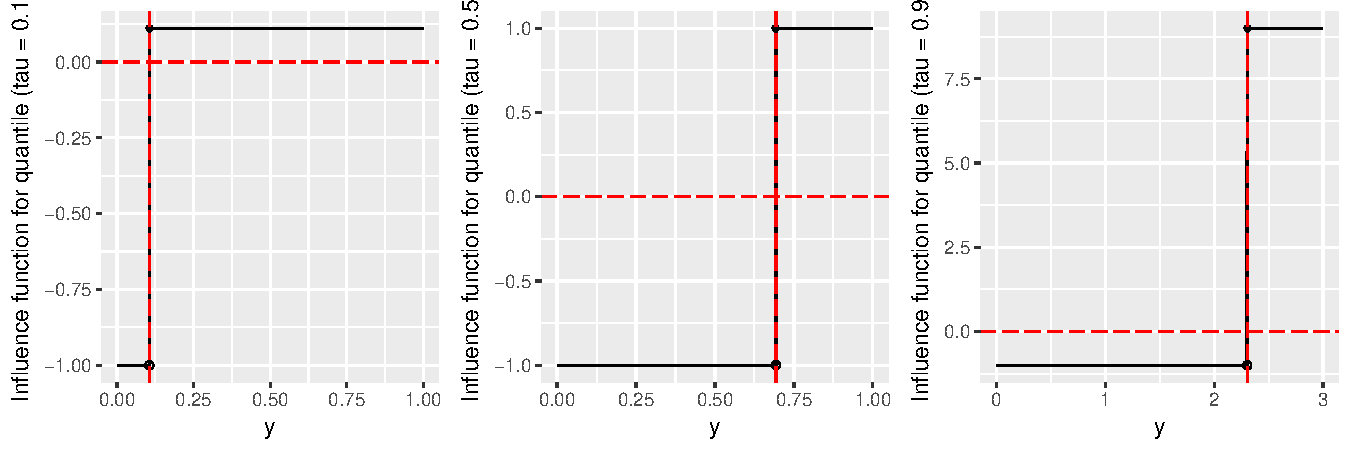
\includegraphics{Diagnosing_outliers_and_visualization_of_quantile_regression_models_files/figure-latex/vis-if-1} 

}

\caption[Visualization of influence function for Mean and Quantile]{Visualization of influence function for Mean and Quantile. It is obviously that quantile influence functions on quantile 0.1, 0.5 and 0.9 are bounded which indicat that quantile is more robust then Mean. The boundaries of influence function on low and high quantile are asymmetrical.}\label{fig:vis-if}
\end{figure}
\end{CodeChunk}

For quantile regression, suppose \(F\) represent the joint distribution
of the pairs \((x,y)\), the influence function is Equation
\eqref{eq:quantile-regression-influence}. Equation
\eqref{eq:quantile-regression-influence} implies that quantile regression
estimates will not be affected by changes in value of dependent variable
as long as the relative positions of the observation points to the
fitted plane are maintained.

\begin{equation}
IF((y,x),\hat{\beta}_{F(\tau)},F)=Q^{-1}x\text{sgn}(y-x^{'}\hat{\beta}_{F}(\tau))
\label{eq:quantile-regression-influence}
\end{equation}

where

\begin{equation}
dF=dG(x)f(y|x)dy
\label{eq: dg}
\end{equation}

\begin{equation}
Q=\int xx^{'}f(X^{'}\hat{\beta}_{F}(\tau))dG(x)
\label{eq:q_influence}
\end{equation}

To illustrate the model robustness indicated by influence function, we
conduct the following simulation study.

\begin{itemize}
\tightlist
\item
  Fitting model with data condaminated by outliers
\end{itemize}

We generate 100 sample observation and 3 outliers to see the relation
between outlier location and the change of coefficients. The outliers
are located at top-left and bottom-right of the original data. Figure
\ref{fig:qr-outlier} show that the former pulled up the regression lines
on quantile 0.9 and 0.5, and the latter pulled down them.

\begin{CodeChunk}
\begin{figure}

{\centering 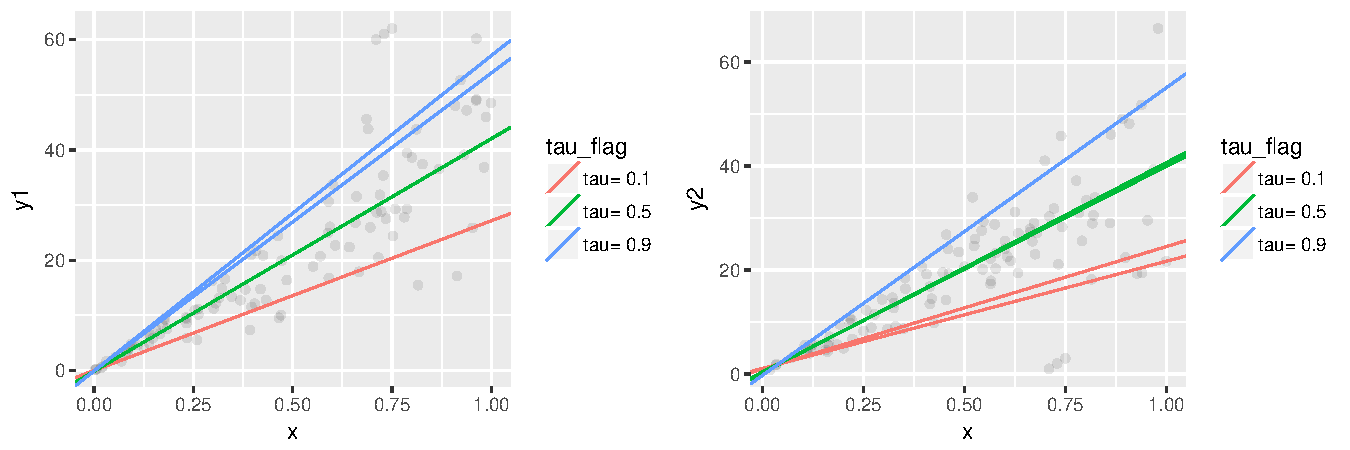
\includegraphics{Diagnosing_outliers_and_visualization_of_quantile_regression_models_files/figure-latex/qr-outlier-1} 

}

\caption[Fitting quantile regression model on quantile 0.1, 0.5 and 0.9 using simulated datasets with and without outliers]{Fitting quantile regression model on quantile 0.1, 0.5 and 0.9 using simulated datasets with and without outliers. The outliers located at the top-left of the original dataset. Results show that outliers pull up the slope of the 0.9 and 0.1 regression line. When outliers located at the bottom-right of the original dataset, results show that outliers pull down the slope of the 0.1 regression line.}\label{fig:qr-outlier}
\end{figure}
\end{CodeChunk}

\begin{itemize}
\tightlist
\item
  Moving outliers location in Y-aixs and X-aixs
\end{itemize}

To visualize the robustness of quantile regression, we simulate 100 data
with 5 condaminated points considered as outliers. We conduct two
experiments to test the boundness of quantile regression towards
outliers. The first experiment is moving outliers in Y-aixs to observe
the change of regression estimated coefficients, and the other is moving
them in X-aix. In the former experiment, Figure \ref{fig:move-y2} show
that when outliers moving down in Y-aixs for 10 unit, they pull down the
slope on every quantile (Comparing the result of \(y_{1}=x+\epsilon\)
and \(y_{2}=x+\epsilon\)). However, figure \ref{fig:move-y2} also show
that keeping moving down the outliers does no change to the regression
slopes. This reflect the boundness of influence function and the
robustness of quantile regression. To observed the change of
coefficients in multi-variable model, we fit quantile regression model
\(y=x_{1}+x_{2}+\epsilon\). Figure \ref{fig:move-y-multi1} show that
coefficients changes slowly when moving down the outliers in Y-axis. In
the other experiment, we follow the similar procedure above while moving
outliers in X-axis. Figure \ref{fig:move-x1} and Figure
\ref{fig:move-x2} show estimated coefficients change every time outliers
move in X-aixs, and the isolate outliers are, the greater of the change.
Besides every move has different effect on each quantiles.

In conclusion, quantile regression response differently to outliers
comparing mean regression in three aspects: (a) not all models on each
quantile will be affected when outliers exist. If we are interested in
model on particular quantile, the effect of outliers should be carefully
considered; (b) the effect of outliers in Y-aixs on quantile regression
has boundary; (c) quantile regression have weak robustness to leverage
points.

\begin{CodeChunk}
\begin{figure}

{\centering 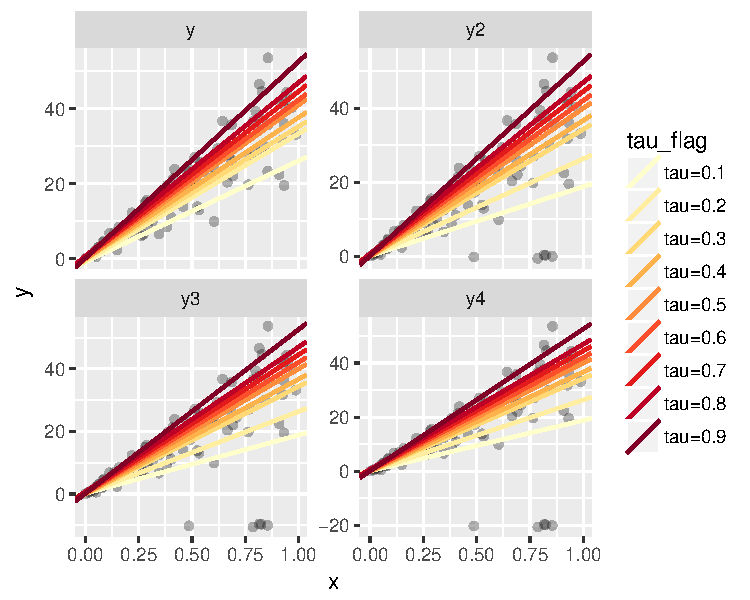
\includegraphics{Diagnosing_outliers_and_visualization_of_quantile_regression_models_files/figure-latex/move-y1-1} 

}

\caption[Fit quantile regression models using simulated data]{Fit quantile regression models using simulated data. Keep moving down the outliers in Y-axis to get different longitudinal ordinates values: $y_{2}=y-5, y_{3}=y-10$ and $y_{4}=y-15$. We are interested in the change of regression lines.}\label{fig:move-y1}
\end{figure}
\end{CodeChunk}

\begin{CodeChunk}
\begin{figure}

{\centering 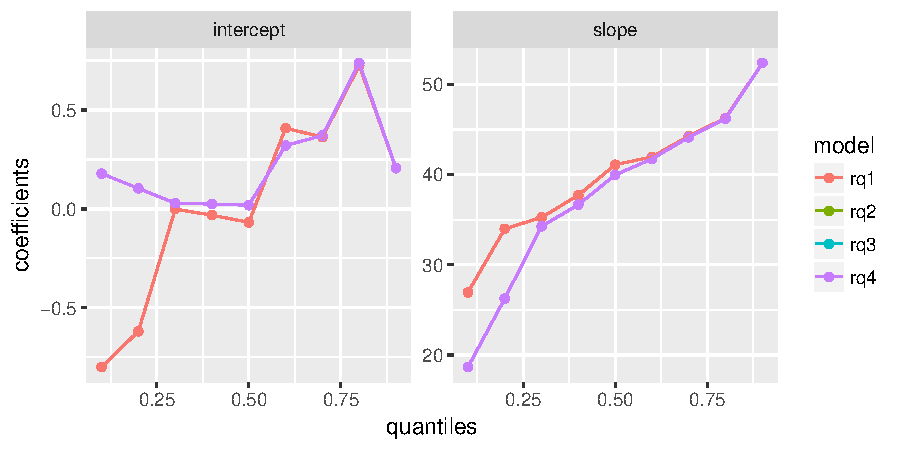
\includegraphics{Diagnosing_outliers_and_visualization_of_quantile_regression_models_files/figure-latex/move-y2-1} 

}

\caption[Fit quantile regression models using simulated data]{Fit quantile regression models using simulated data. Keep moving down the outliers in Y-axis to get different longitudinal coordinates values: $y_{2}=y-5, y_{3}=y-10$ and $y_{4}=y-15$. Calculating the estimated coefficients in each experiment and results show that in single predictor case, outliers moving down in y make no difference to the quantile regression coefficients estimations. This visualization show the bound property of influence function for quantile regression.}\label{fig:move-y2}
\end{figure}
\end{CodeChunk}

\begin{CodeChunk}
\begin{figure}

{\centering 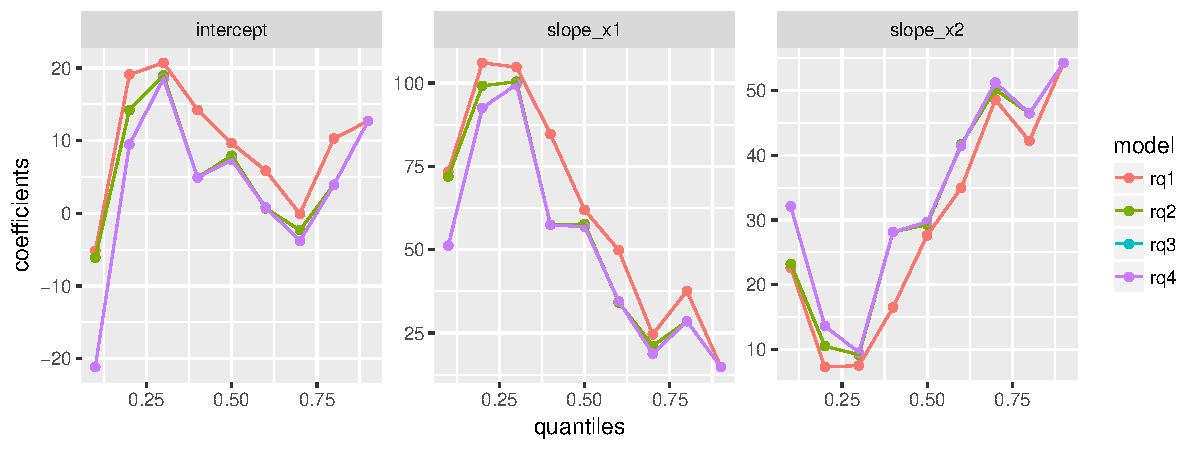
\includegraphics{Diagnosing_outliers_and_visualization_of_quantile_regression_models_files/figure-latex/move-y-multi1-1} 

}

\caption[Fit quantile regression models using simulated data]{Fit quantile regression models using simulated data. Keep moving down the outliers in Y-axis to get different longitudinal coordinates values: $y_{2}=y-5, y_{3}=y-10$ and $y_{4}=y-15$. Results show that in multi predictors case, outliers moving down in Y-axis still makes little change to the quantile regression coefficients estimations.}\label{fig:move-y-multi1}
\end{figure}
\end{CodeChunk}

\begin{CodeChunk}
\begin{figure}

{\centering 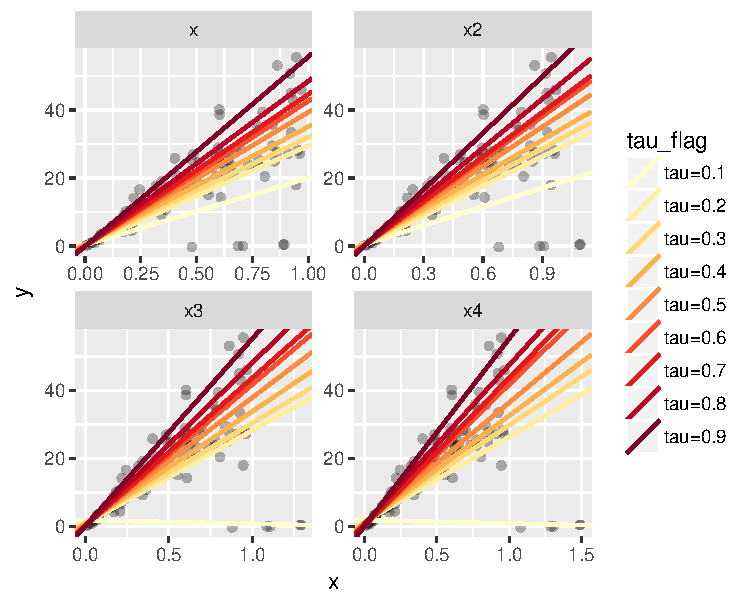
\includegraphics{Diagnosing_outliers_and_visualization_of_quantile_regression_models_files/figure-latex/move-x1-1} 

}

\caption{Fit quantile regression models using simulated data. Keep moving the outliers to the right in X-aixs to get different horizontal ordinate values: $x_{2}=x+0.2, x_{3}=x+0.4$ and $x_{4}=x+0.6$. We are interested in the change of regression lines.}\label{fig:move-x1}
\end{figure}
\end{CodeChunk}

\begin{CodeChunk}
\begin{figure}

{\centering 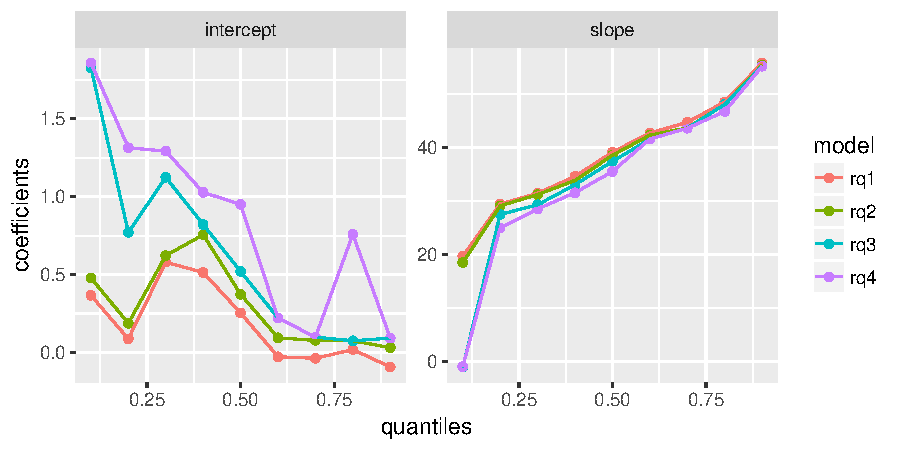
\includegraphics{Diagnosing_outliers_and_visualization_of_quantile_regression_models_files/figure-latex/move-x2-1} 

}

\caption{Fit quantile regression models using simulated data. Keep moving the outliers to the right in X-aixs to get different horizontal ordinate values: $x_{2}=x+0.2, x_{3}=x+0.4$ and $x_{4}=x+0.6$. Calculating the estimated coefficients in each experiment and results show that outliers moving in X-aixs make larger difference to the quantile regression coefficients then moving in Y-aixs.}\label{fig:move-x2}
\end{figure}
\end{CodeChunk}

\section{Outlier Diagnostic Methods for Quantile
Regression}\label{outlier-diagnostic-methods-for-quantile-regression}

In this section we briefly introduce diagnostic methods used in
\texttt{quokar}. These methods are well discussed in recent literatures
(\citet{sanchez2013likelihood}, \citet{santos2016bayesian}) and
performed well in our application. We assume a basic knowledge of
quantile regerssion and Baysian methods.

\subsection{Residual-Robust Distance}\label{residual-robust-distance}

In quantile regression, we can not use the famous ``Hat Matrix'' to
detect leverage points since the coefficient estimation of quantile
regression do not satisfy \(\hat{\beta}=(X^{'}X)^{-1}X^{'}Y\). One way
to identify possible leverage points is to calculate a distance from
each point to a ``center'' of the data. Leverage point would then be the
one with a distance larger than some predetermined cutoff. A
conventional measurement is Mahalanobi distance:

\begin{equation}
MD(x_i) = [(x_i-\bar{x})^{'}\bar{\boldsymbol{C}}(\boldsymbol{X})^{-1}(x_i-\bar{x})]^{1/2}
\label{eq:distance}
\end{equation}

where \(\bar{x}=\frac{1}{n}\sum_{i=1}^{n}x_i\) and
\(\bar{\boldsymbol{C}}(\boldsymbol{X})=\frac{1}{n-1}\sum_{i=1}^{n}(x_i-\bar{x})^{'}(x_i-\bar{x})\)
are the empirical multivariate location and scale respectively. However,
the standard sample location and scale parameters are not robust to
outliers. In addition, datasets with multiple outliers or clusters of
outliers are subject to problems of masking and swamping
(\citet{pearson1936efficiency}). Such problems of unrobust, masking and
swamping can be resolved by using robust estimates of shape and
location, which by definition are less affected by outliers
(\citet{rousseeuw1991robust}). In quokar, we use minimum covariance
determinant (MCD) proposed by \citet{rousseeuw1999fast} to estimate the
above two parameters. The MCD estimator can be defined as

\begin{equation}
MCD = (\bar{X}^{*}_{h}, S^{*}_{h})
\label{eq: mcd}
\end{equation}

where \(\bar{X}\) and \(S\) represent location and scale.
\(h={p: |S^{*}_{h}|<|S^{*}_{k}|,|k|=p}\),
\(\bar{X}^{*}_{h}=\frac{1}{p}\sum_{i \in p}x_{i}\),
\(S^{*}_{p}=\frac{1}{p}\sum_{i \in p}(x_i-\bar{X}^{*}_{p})(x_i-\bar{X}^{*}_{p})^{'}\).
\(p\) can be thought as the minimum number of points which must not be
outliers. The MCD has its highest possible breakdown at
\(h=[\frac{n+p+1}{2}]\) where \([.]\) is the greatest integer function.
Because we are interested in outlier detection, we will use \(h\) at its
highest possible breakdown. With MCD, we can calculate robust distance
which was defined as

\begin{equation}
RD(x_i)=[(x_i-\boldsymbol{T(A)})^{'}\boldsymbol{C(A)}^{-1}(x_i-\boldsymbol{T(A)})]^{1/2}
\label{eq:rd}
\end{equation}

Where \(\boldsymbol{T(X)}\) and \(\boldsymbol{C(X)}\) are robust
multivariate location and scale estimates that are computed according to
the MCD.

Package \texttt{quokar} implement Mahalanobi distance and robust
distance to detect leverage points in quantile regression. Residuals
that are based on quantile regression estimates are used to detect
vertical outliers.

\subsection{Cook's Distance and Likelihood
Distance}\label{cooks-distance-and-likelihood-distance}

Case-deletion diagnostics such as Cook's distance or Likelihood distance
have been successfully applied to various statistical models. Based on
the research of \citet{sanchez2013likelihood}, we calculate Cook's
distance and Likelihood distance for quantile regression in package
\texttt{quokar}. More specify process will be discussed as follows.

\citet{yu2001bayesian} proposed random variable \(Y\) distributed as
asymmetric Laplace distribution with location parameter \(\mu\), scale
parameter \(\sigma >0\) and skewness parameter \(\tau \in (0,1)\) has
density function:

\begin{equation}
f(y|\mu, \sigma, \tau) = \frac{\tau (1-\tau)}{\sigma}exp\{-\rho_{p}(\frac{(y-\mu)}{\sigma})\}
\label{eq: ald}
\end{equation}

where \(\rho_{\tau}(.)\) is the loss function mentioned above. Suppose
that
\(y_i \sim ALD(\boldsymbol{x}^{'}_{i}\mathbf{\beta}_{p}, \sigma, \tau)\),
\(i=1,...,n\) are independent. The likelihood function for \(n\)
observations is

\begin{equation}
L(\mathbf{\beta},\sigma|y)=\frac{\tau^{n}(1-\tau)^{n}}{\sigma^{n}}exp\{-\sum_{i=1}^{n} \rho_{\tau}(\frac{y_i-\boldsymbol{x}^{'}_{i}}{\sigma})\}
\label{eq:ald_likelihood}
\end{equation}

For note, a quantity with a subscript \([i]\) means the relevant
quantity with the \(i\)th observation deleted. Let \(\hat{\theta}\) and
\(\hat{\theta}^{*}_{[i]}\) be the maximum likelihood estimator of
\(\theta\) based on \(L(\theta|Y)\) and \(L(\theta|Y_{[i]})\)
respectively. Cook's distance \(CD_{i}\) is given by \eqref{eq:cd}. For
external norms, \(M\) is usually chosen to be \(-\ddot{L}(Y|\theta)\).

\begin{equation}
CD_{i}=(\hat{\theta}^{*}_{[i]}-\hat{\theta})^{'}M(\hat{\theta}^{*}_{[i]}-\hat{\theta})
\label{eq:cd}
\end{equation}

Alternatively, another measure of difference between \(\theta\) and
\(\theta^{*}_{[i]}\) is the observed data likelihood function which is
defined as Likelihood distance.

\begin{equation}
LD_i=L(\hat{\theta}|Y)-L(\hat{\theta}^{*}_{[i]}|Y)
\label{eq: ld}
\end{equation}

The \(i\)th observation is regarded as influential if the value of
Cook's distance or likelihood distance is relatively large.
\citet{benites2015case} proposed a EM algorithm to calculate the above
Cook's distance and likelihood distance which reduced the calculation
burden. They used the expectation of likelihood function (Equation
q\_function) for estimation.

\begin{equation}
Q(\theta|\hat{\theta})=E\{L(\theta|Y)|\hat{\theta}\}
\label{eq:q_function}
\end{equation}

To assess the influence of the \(i\)th case, we will consider the
function

\begin{equation}
Q_{[i]}(\theta|\hat{\theta})=E\{L(\theta|Y_{[i]})|\hat{\theta}\}
\label{eq: q_one_deletion}
\end{equation}

Let \(\hat{\theta}_{[i]}\) be the maximiser of
\(Q_{[i]}(\theta|\hat{\theta})\). The one-step approximation
\(\hat{\theta}_{[i]}\) is

\begin{equation}
\hat{\theta}_{[i]}=\hat{\theta}+\{-\ddot{Q}(\hat{\theta}|\hat{\theta})\}^{-1}\dot{Q}_{[i]}(\hat{\theta}|\hat{\theta})
\label{eq: estimator}
\end{equation}

where

\[\dot{Q}_{[i]}(\hat{\theta}|\hat{\theta})=\frac{\partial Q_{[i]}(\theta|\hat{\theta})}{\partial\theta}|_{\theta=\hat{\theta}}\]

\[\ddot{Q}(\hat{\theta}|\hat{\theta})=\frac{\partial^{2}Q(\theta|\hat{\theta})}{\partial\theta\partial \theta^{'}}|_{\theta=\hat{\theta}}\]

are the Hessian matrix and the gradient vector evaluated at
\(\hat{\theta}\) respectively.

Hence, the Cook's distance is defined as

\begin{equation}
CD_{i} =(\hat{\theta}_{[i]}-\hat{\theta})^{'}\{-Q(\hat{\theta}|\hat{\theta})\}(\hat{\theta}_{[i]}-\hat{\theta}), \quad i=1,...,n
\label{eq:gd}
\end{equation}

The measurement of the influence of the \(i\)th case which based
directly on the Q function is similar to the likelihood distance
\(LD_{i}\). It can be defined as,

\begin{equation}
QD_{i}=2\{Q(\hat{\theta}|\hat{\theta})-Q(\hat{\theta}_{[i]}|\hat{\theta})\} \quad i=1,...,n
\label{eq:qd}
\end{equation}

\subsection{Mean Posterior Probability and Kullback-Leibler
Divergence}\label{mean-posterior-probability-and-kullback-leibler-divergence}

In Bayesian quantile regression framework,
\citet{kullback1951information} proposed a location-scale mixture
representation of the asymmetric Laplace distrbution, as follows,

\begin{equation}
Y|v \sim N(\mu + \theta v, \phi^{2}\sigma v)
\label{eq:mixture}
\end{equation}

where \(\theta=(1-2\tau)/(\tau(1-\tau))\),
\(\phi^{2}=2/(\tau(1-\tau))\). \(v\) is a latent variable which prior
distribution is exponential and the full conditional posterior
distribution for each \(vi\) follows generalized inverse Gaussian
distribution with parameters,

\begin{equation}
v=\frac{1}{2}, \quad \delta^{2}_{i}=\frac{(y_i-x^{'}_{i}\beta(\tau))^{2}}{\phi^{2}\sigma}, \quad 
\gamma^2=\frac{2}{\sigma}+\frac{\theta^{2}}{\phi^{2}\sigma}
\label{eq:parameters}
\end{equation}

Parameters of \(v_i\) in \eqref{eq:parameters} show two characters of
latent variable \(v\): (a) each random variable \(v_i\) has different
distributions due to parameter \(\delta^2\) changes among obvervations.
(b) distribution of \(v_i\) depended on weighted squared residual of the
quantile fit. Based on the above two characters, we propose to compare
the posterior distribution of its latent variable to detect outliers. We
implete two methods in \texttt{quokar}, one is mean posterior prability
and the other is Kullback-Leibler divergence. We define variable \(O_i\)
indicating whether observation \(i\) is an outlier.

\begin{equation}
O_i = \left\{
\begin{aligned}
1 & , & i \quad is \quad outlier \\
0 & , & i \quad is \quad normal
\end{aligned}
\right.
\label{eq:indicating_outlier}
\end{equation}

The mean posterior probability appoximatlly calculated by MCMC draw is

\begin{equation}
P(O_i = 1)=\frac{1}{n-1}\sum_{j \neq i}\frac{1}{M}I(v^{(l)}_{i}> \text{max}_{k \in 1:M}v^{(k)}_j)
\label{eq:mcmc_draw}
\end{equation}

where \(M\) is the size of the chain of \(v_i\) after the burn-in perior
and \(v^{(l)}_i\) is the \(l\)th draw of this chain.
\citet{kullback1951information} proposed a more precise method of
measuring the distance between variables. Suppose \(f_i\) is the
posterior conditional distribution of \(v_i\) and correspondingly
\(f_j\) is the posterior conditional distribution of \(v_j\). The
Kullback-Leibler divergence of \(f_i\) and \(f_j\) is defined in
Equation @ref(eq:kl\_divergence) and @ref(eq:mean\_posterior\_kl). The
outliers should show a high probability value for this divergence. We
compute the integral using the trapezoidal rule, and the density
function are estimated using kernel estimation with Gaussian kernel
function.

\begin{equation}
K(f_i, f_j)=\int log(\frac{f_i(x)}{f_j(x)})f_{i}(x)dx
\label{eq:kl_divergence}
\end{equation}

Similar with calculating mean posterior probability, we average this
divergence for one observation based on the distance from all others,

\begin{equation}
KL(f_i)=\frac{1}{n-1}\sum_{j\neq i}K(f_i, f_j)
\label{eq:mean_posterior_kl}
\end{equation}

\section{Examining Outlier Detection}\label{examining-outlier-detection}

We developed R package \texttt{quokar} to implete quantile regression
outlier diagnostic methods. This package mainly realized two basic
features: (a) plot the outlier state; (b) plot data with outliers
marked. \texttt{quokar} is available from Github at
\url{https://github.com/wenjingwang/quokar}, so to install and load
withn R use:

\begin{CodeChunk}

\begin{CodeInput}
R> devtools::install_github("wenjingwang/quokar")
R> library(quokar)
\end{CodeInput}
\end{CodeChunk}

We implete Australia Institution of Sports (AIS) data as an example to
introduce this package. AIS is a data frame with 202 observations (102
male and 100 female) on 13 variables. The female data contain outlier
which suit for our research.

\subsection{Plot the outlier state}\label{plot-the-outlier-state}

In single variable case, we can use scatter plot to represent the
outlier state. The following code showed how to display suspicious
outliers based on quantile regression models. Figure
\ref{fig:single-case} showed the potential outlier is case 1 and 75.
When comes to multi-variable case, one way to display the outlier state
in data by the scatter plot on separate covariants. Figure
\ref{fig:multi-case} showed case 56 and 75 are suspicious outliers in
the data set.

\begin{CodeChunk}

\begin{CodeInput}
R> data(ais)
R> ais_female <- filter(ais, Sex == 1)
R> case <- 1 : nrow(ais_female)
R> ais_female <- cbind(case, ais_female)
R> coef_rq <- coef(rq(BMI ~ LBM, tau = c(0.1, 0.5, 0.9),
R+                    data = ais_female, method = "br"))
R> 
R> br_coef <- data.frame(intercept = coef_rq[1, ],
R+                       coef = coef_rq[2, ],
R+                       tau_flag = colnames(coef_rq))
R> ggplot(ais_female)+
R+   geom_point(aes(x = LBM, y = BMI)) +
R+   geom_abline(data = br_coef, aes(intercept = intercept,
R+                                   slope = coef,
R+                                   colour = tau_flag), size = 1) +
R+   geom_text(data = subset(ais_female, case %in% c(1, 75)),
R+                           aes(x = LBM, y = BMI, label = case), 
R+             colour = "red",hjust = 0, vjust = 0) +
R+   scale_colour_brewer(palette="YlOrRd")+
R+   theme_grey()
\end{CodeInput}
\begin{figure}

{\centering 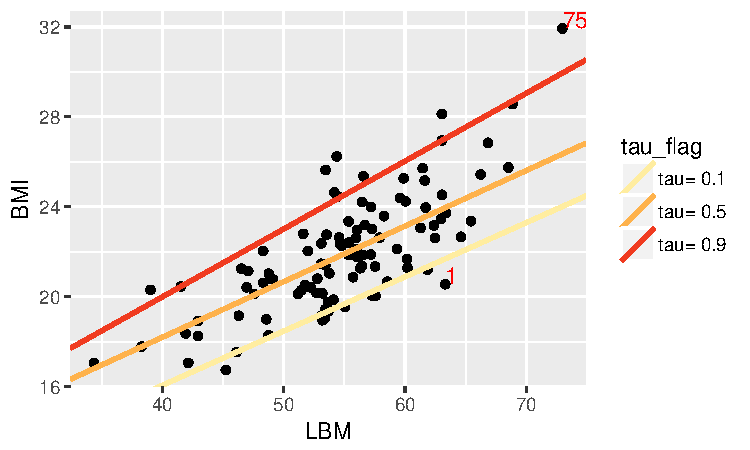
\includegraphics{Diagnosing_outliers_and_visualization_of_quantile_regression_models_files/figure-latex/single-case-1} 

}

\caption[Plot the outlier state for single variable case]{Plot the outlier state for single variable case.}\label{fig:single-case}
\end{figure}
\end{CodeChunk}

\begin{CodeChunk}

\begin{CodeInput}
R> ais_female_f <- dplyr::select(ais_female, c(case, BMI, LBM, Bfat))
R> ais_female_f_long <- tidyr::gather(ais_female_f, variable, value, -case, -BMI)
R> ggplot(ais_female_f_long, aes(x = value, y = BMI))+
R+   geom_point(alpha = 0.5) +
R+   geom_text(data = subset(ais_female_f_long, case %in% c(56, 75)),
R+                           aes(x = value, y = BMI, label = case), 
R+             colour = "red", vjust = 0, hjust = 0) +
R+   facet_wrap(~variable, scales = "free_x") +
R+   scale_colour_brewer(palette="YlOrRd")+
R+   theme_grey()
\end{CodeInput}
\begin{figure}

{\centering 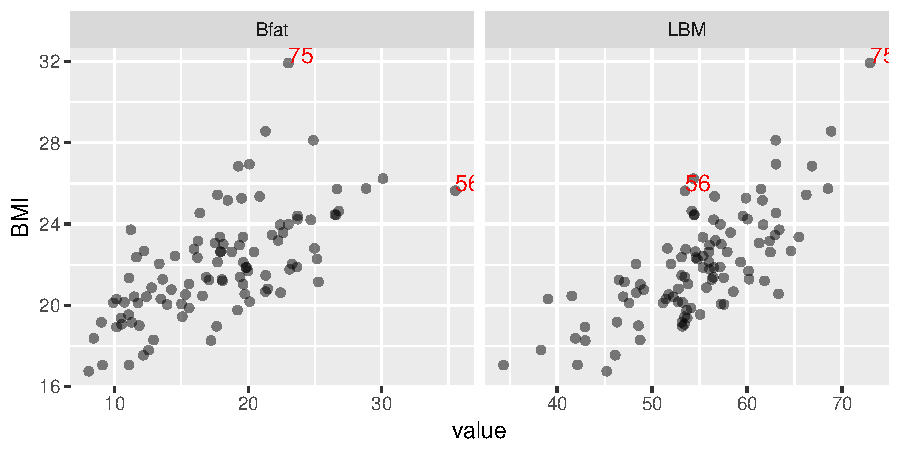
\includegraphics{Diagnosing_outliers_and_visualization_of_quantile_regression_models_files/figure-latex/multi-case-1} 

}

\caption[Plot the outlier state for multi-variable regression]{Plot the outlier state for multi-variable regression.}\label{fig:multi-case}
\end{figure}
\end{CodeChunk}

\subsection{Plot data with outliers
marked}\label{plot-data-with-outliers-marked}

Scatter plot has limitations when tackling multi-variable regression. In
\texttt{quokar}, we provide functions to do outlier diagnostic which
return the dataframe easily to plot data with outliers marked.

\begin{itemize}
\tightlist
\item
  residual-robust distance method
\end{itemize}

First, we calculate residuals, mahananobi distance and robust distance
for quantile regression using function \texttt{plot\_distance}.
Simutaneously, it provides the cutoff value for identifying the
outliers.

\begin{CodeChunk}

\begin{CodeInput}
R> tau <- c(0.1, 0.5, 0.9)
R> object <- rq(BMI ~ LBM + Bfat, data = ais_female, tau = tau)
R> plot_distance <- frame_distance(object, tau = c(0.1, 0.5, 0.9))
R> distance <- plot_distance[[1]]
R> head(distance, 3)
\end{CodeInput}

\begin{CodeOutput}
         md        rd tau_flag  residuals
1 1.2275233 1.3912428   tau0.1 -1.4630550
2 0.6988854 0.6486756   tau0.1 -0.9262022
3 0.3836449 0.3315911   tau0.1  1.0706377
\end{CodeOutput}

\begin{CodeInput}
R> cutoff_v <- plot_distance[[2]]; cutoff_v
\end{CodeInput}

\begin{CodeOutput}
[1] 2.716203
\end{CodeOutput}

\begin{CodeInput}
R> cutoff_h <- plot_distance[[3]]; cutoff_h
\end{CodeInput}

\begin{CodeOutput}
[1] 12.450378  6.917875 14.073312
\end{CodeOutput}
\end{CodeChunk}

Function \texttt{plot\_distance} returns the tidy data form for plotting
data with outliers marked together overlaying the cutoff lines. We use
the following code for visualizing the diagnose result. Figure 8 showed,
on quantile 0.1, 0.5 and 0.9, case 56, 75, 98 and 100 are detected as
leverage points and no outliers in y-direction exsited.

\begin{CodeChunk}

\begin{CodeInput}
R> n <- nrow(object$model)
R> case <- rep(1:n, length(tau))
R> distance <- cbind(case, distance)
R> distance$residuals <- abs(distance$residuals)
R> tau_f <- paste("tau", tau, sep="")
R> text_flag <- 1:length(cutoff_h) %>%
R+                     map(function(i){
R+                         distance %>% 
R+                            filter((residuals > cutoff_h[i] |rd > cutoff_v)
R+                                 & tau_flag == tau_f[i])})
R> 
R> text_flag_d <- rbind(text_flag[[1]], text_flag[[2]], text_flag[[3]])
R> ggplot(distance, aes(x = rd, y = residuals)) +
R+       geom_point() +
R+       geom_hline(data = data.frame(tau_flag = paste("tau", tau, sep=""), 
R+                                    cutoff_h = cutoff_h),   
R+                  aes(yintercept = cutoff_h), colour = "red") +
R+       geom_vline(xintercept = cutoff_v, colour = "red") +
R+       geom_text(data = text_flag_d, aes(label = case), hjust = 0, vjust = 0) +
R+       facet_wrap(~ tau_flag, scales = 'free_y') +
R+       xlab("Robust Distance") +
R+       ylab("|Residuals|")
\end{CodeInput}
\begin{figure}

{\centering 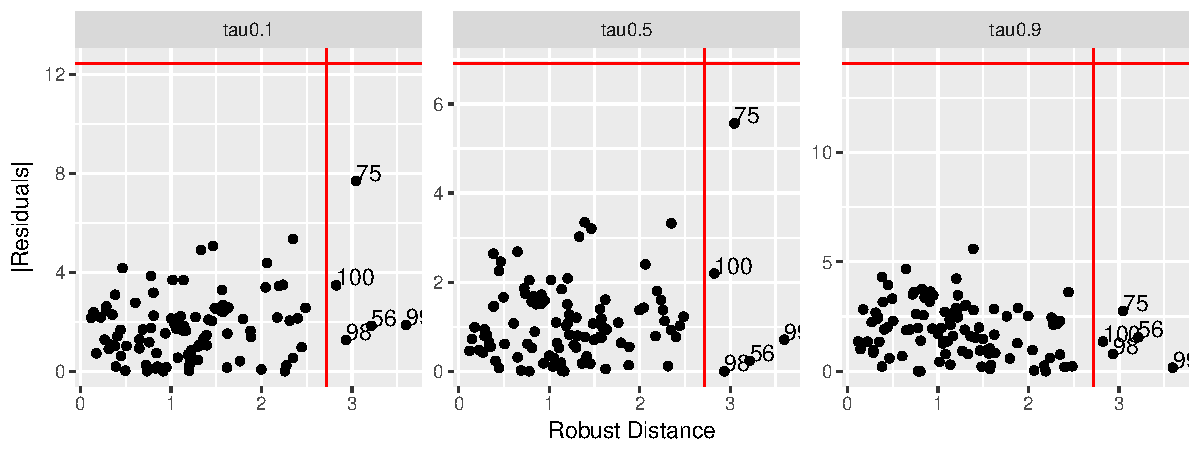
\includegraphics{Diagnosing_outliers_and_visualization_of_quantile_regression_models_files/figure-latex/unnamed-chunk-4-1} 

}

\caption[Robust Distance-Residual Plot]{Robust Distance-Residual Plot. Points on the right of vertical cutoff line are considered leverage points and points above the horizental cutoff line are outliers in y-direction.}\label{fig:unnamed-chunk-4}
\end{figure}
\end{CodeChunk}

* Generalized Cook distance and Q function distance

We apply generalized Cook distance and Q function distance methods in function \code{frame_mle} using AIS data. Methods \code{bayes.prob} and \code{bayes.kl} in function \code{frame_bayes} return the mean probability and Kullback-Leibler divergence of each observation on each given quantile. The results are also in tidy data structure which can be easily used for plotting the two distances with outliers marked. Figure 9 and 10 show regression model on 0.1 quantile has outlier case 1, and case 75 is the potential outlier of regression models on quantile 0.5 and 0.9. 

\begin{CodeChunk}

\begin{CodeInput}
R> y <- ais_female$BMI
R> x <- cbind(1, ais_female$LBM, ais_female$Bfat)
R> case <- rep(1:length(y), length(tau))
R> GCD <- frame_mle(y, x, tau, error = 1e-06, iter = 10000,
R+                   method = 'cook.distance')
R> GCD_m <- cbind(case, GCD)
R> ggplot(GCD_m, aes(x = case, y = value )) +
R+     geom_point() +
R+     facet_wrap(~variable, scale = 'free_y') +
R+     geom_text(data = subset(GCD_m, value > mean(value) + 2*sd(value)),
R+               aes(label = case), hjust = 0, vjust = 0) +
R+     xlab("case number") +
R+     ylab("Generalized Cook Distance")
\end{CodeInput}
\begin{figure}

{\centering 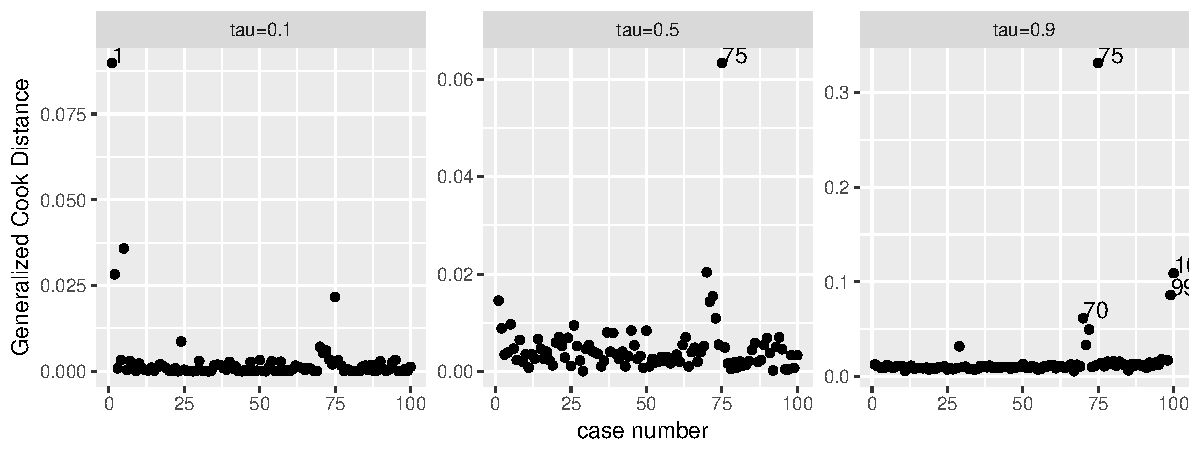
\includegraphics{Diagnosing_outliers_and_visualization_of_quantile_regression_models_files/figure-latex/unnamed-chunk-5-1} 

}

\caption[Generalized Cook distance of each observation on quantile 0.1, 0.5 and 0.9]{Generalized Cook distance of each observation on quantile 0.1, 0.5 and 0.9. Case 75 has relative large Cook distance-funtion distance to other points}\label{fig:unnamed-chunk-5}
\end{figure}
\end{CodeChunk}\begin{CodeChunk}

\begin{CodeInput}
R> QD <- frame_mle(y, x, tau, error = 1e-06, iter = 10000,
R+                method = 'qfunction')
R> QD_m <- cbind(case, QD)
R> ggplot(QD_m, aes(x = case, y = value)) +
R+  geom_point() +
R+  facet_wrap(~variable, scale = 'free_y')+
R+  geom_text(data = subset(QD_m, value > mean(value) + sd(value)),
R+            aes(label = case), hjust = 0, vjust = 0) +
R+  xlab('case number') +
R+  ylab('Qfunction Distance')
\end{CodeInput}
\begin{figure}

{\centering 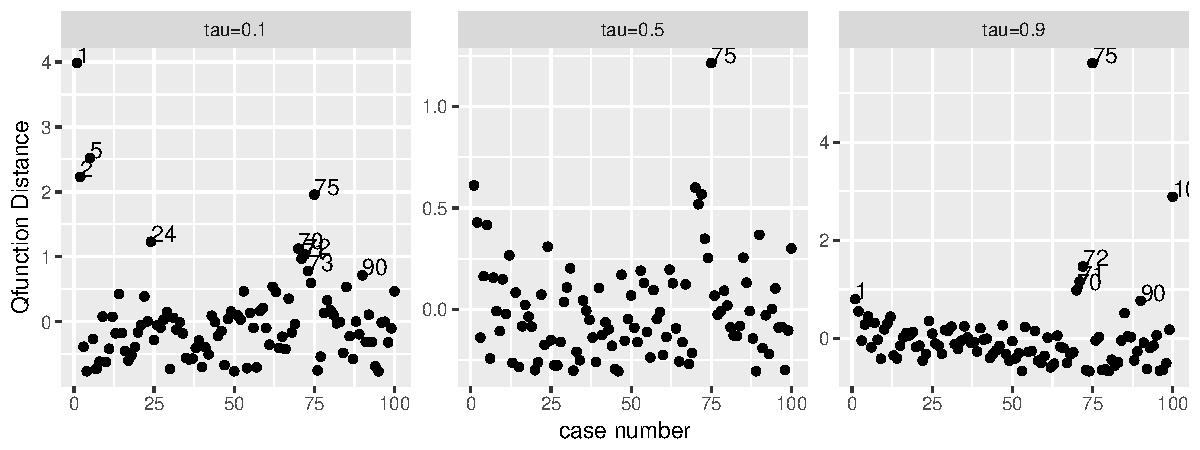
\includegraphics{Diagnosing_outliers_and_visualization_of_quantile_regression_models_files/figure-latex/unnamed-chunk-6-1} 

}

\caption[Q function distance of each observation on quantile 0.1, 0.5 and 0.9]{Q function distance of each observation on quantile 0.1, 0.5 and 0.9. Case 75 has relative large Q function distance to other points}\label{fig:unnamed-chunk-6}
\end{figure}
\end{CodeChunk}

\textbackslash{}begin\{CodeChunk\}

\textbackslash{}begin\{CodeInput\} R\textgreater{} y \textless{}-
ais\_female\(BMI R> x <- matrix(c(ais_female\)LBM, ais\_female\$Bfat),
ncol = 2, byrow = FALSE) R\textgreater{} tau \textless{}- c(0.1, 0.5,
0.9) R\textgreater{} case \textless{}- rep(1:length(y), length(tau))
R\textgreater{} prob \textless{}- frame\_bayes(y, x, tau, M = 5000, burn
= 1000, R\textgreater{} method = `bayes.prob') R\textgreater{}
R\textgreater{} kl \textless{}- frame\_bayes(y, x, tau, M = 5000, burn =
1000, R\textgreater{} method = `bayes.kl')
\textbackslash{}end\{CodeInput\} \textbackslash{}end\{CodeChunk\}

\begin{CodeChunk}

\begin{CodeInput}
R> head(prob)
R> head(kl)
\end{CodeInput}
\end{CodeChunk}

With the result which is long data form returned by function
\code{frame_bayes}, we provide visualization of the mean posterior
probability and Kullback-Leibler divergence of each observation with
outlier marked. Figure 11 and 12 show that the potential outlier is case
75.

\begin{CodeChunk}

\begin{CodeInput}
R> prob_m <- cbind(case, prob)
R> ggplot(prob_m, aes(x = case, y = value )) +
R>    geom_point() +
R>    facet_wrap(~variable, scale = 'free') +
R>   geom_text(data = subset(prob_m, value > mean(value) + 2*sd(value)),
R>             aes(label = case), hjust = 0, vjust = 0) +
R>    xlab("case number") +
R>    ylab("Mean probability of posterior distribution")
\end{CodeInput}
\end{CodeChunk}

\begin{CodeChunk}

\begin{CodeInput}
R> kl_m <- cbind(case, kl)
R> ggplot(kl_m, aes(x = case, y = value)) +
R>   geom_point() +
R>   facet_wrap(~variable, scale = 'free')+
R>   geom_text(data = subset(kl_m, value > mean(value) + sd(value)),
R>             aes(label = case), hjust = 0, vjust = 0) +
R>   xlab('case number') +
R>   ylab('Kullback-Leibler')
\end{CodeInput}
\end{CodeChunk}

\section{Generalized Framework for Visualizing Quantile Regrssion
Model}\label{generalized-framework-for-visualizing-quantile-regrssion-model}

Visualization is particularly useful and comprehensive way to explore
data and model. It is also a extremely straight-forward way to detect
outlier by observing the location of data and model. In regression
context, a fitted regression model is not only judged by its prediction
error, rather other questions worth to consider, such as do the data
space is too inseparablely or too sparesly to be represented by the
data; are there some regions that are difficultly for model to fit. For
quantile regression, we are also curious to know what is the relative
location of models on different quantiles in data space.

Use model visualization to discover useful information in fitted
quantile regression and high dimensional data set is a challenging
problem. There exists no work which aims to visualize the quantile
regression itself. In this section, we propose approach aimed to
visualize the whole data set together with the quantile regression
models fitted on different quantile in one plot. In this way, we can
analyze model fitting, model performance and model comparison
simultaneously.

Given our visualization results, the exploring and observing aspects are
organized into the following steps.

\begin{itemize}
\item
  Is data clustered or sparsely distributed? How do quantile regression
  models deal with that?
\item
  Do model overfit/underfit exist?
\item
  Are there potential outlier exist in the data and how methods treat
  these?
\item
  How do models fitted on different quantiles located in different
  regions of data space?
\item
  What about the relative locations of quantile regression models?
\end{itemize}

Our visualizations are realized by software \texttt{GGobi}
(\citet{swayne2003ggobi}). \texttt{GGobi} is a free software for
interactive and dynamic graphics which can be used with R via package
\texttt{rggobi}. With \texttt{GGobi}, we can extend the limit of 2D
visualization of quantile regression model and break the visualization
barrier in 3D or much higher dimension.

We proposed a feasible framework to visualize quantile regression model
in \texttt{GGobi}. Assumming given data set including points
\(\boldsymbol{x}_{i} \in \boldsymbol{X}\). In high dimension case,
\(\boldsymbol{x}_i\) is a vector and \(\boldsymbol{X}\) is matrix. The
\(i\)th value of responsor \(\boldsymbol{Y}\) is \(y_i\). The quantile
regression model \(f_{\tau}:\boldsymbol{X} \rightarrow \boldsymbol{Y}\)
will be fitted on the given data set.

\begin{itemize}
\item
  Use grid method to generate data in data space bounded by
  \(\boldsymbol{X}\). The generated data form data set
  \(\boldsymbol{Z}\).
\item
  Fit quantile regression models \(f_{\tau}\) on every interested
  quantile and get the estimated parameters \(\bold{\beta}_{\tau}\).
\item
  Calculate quantile regression model using
  \(f_{\tau} = \bold{Z}\bold{\beta}_{\tau}\). In non-linear case,
  calculate model based on the non-linear curve form.
\item
  Tidy data set \((\boldsymbol{Z}, f_{\tau})\) for each quantile into
  long data form and add tag representing quantile.
\end{itemize}

\subsection{Linear Case Result}\label{linear-case-result}

In two predictors case (3D data space), quantile regression models are
planes in space. We use ais data to fit models and visualize them with
\texttt{GGobi}.

\begin{CodeChunk}
\begin{figure}

{\centering 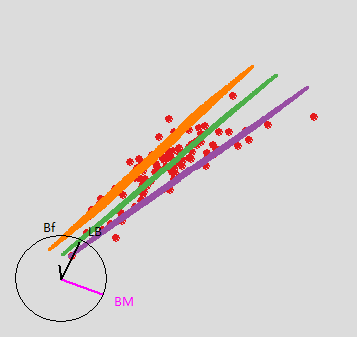
\includegraphics[width=0.25\linewidth]{Figures/QR-model-single-pixel/linear-3D-1} 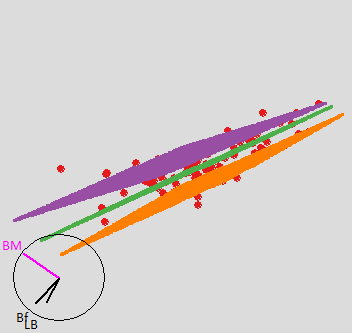
\includegraphics[width=0.25\linewidth]{Figures/QR-model-single-pixel/linear-3D-2} 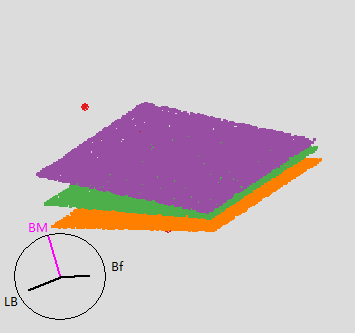
\includegraphics[width=0.25\linewidth]{Figures/QR-model-single-pixel/linear-3D-3} 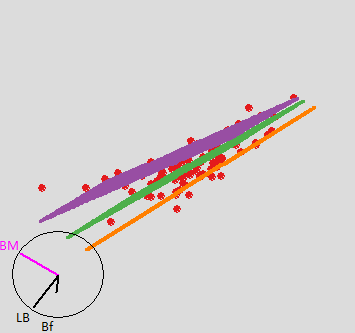
\includegraphics[width=0.25\linewidth]{Figures/QR-model-single-pixel/linear-3D-4} 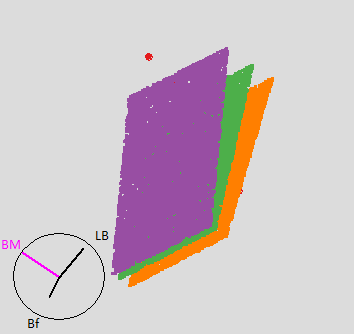
\includegraphics[width=0.25\linewidth]{Figures/QR-model-single-pixel/linear-3D-5} 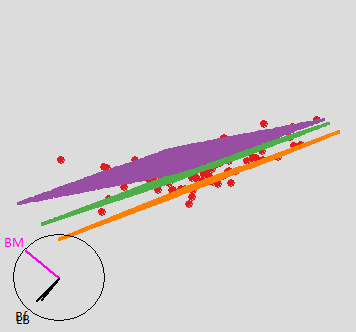
\includegraphics[width=0.25\linewidth]{Figures/QR-model-single-pixel/linear-3D-6} 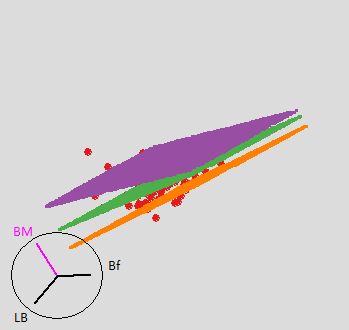
\includegraphics[width=0.25\linewidth]{Figures/QR-model-single-pixel/linear-3D-7} 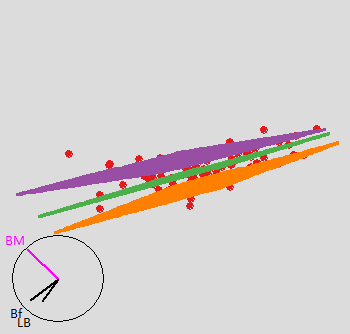
\includegraphics[width=0.25\linewidth]{Figures/QR-model-single-pixel/linear-3D-8} 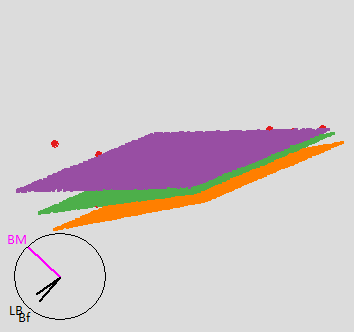
\includegraphics[width=0.25\linewidth]{Figures/QR-model-single-pixel/linear-3D-9} 

}

\caption[Linear quantile regression model with 2 response variables]{Linear quantile regression model with 2 response variables. Models on quantile 0.1, 0.5 and 0.9 corresponds to color orange, green and purple.}\label{fig:fig-name0}
\end{figure}
\end{CodeChunk}

Figure \ref{fig:fig-name0} show that one point is isolated in data space
from other points and three fitted quantile regression models which
indicating this point is potential outliers for the models fitted. The
three quantile regression models are not paralleled in the data space
and they respectively fitted the data set on quantile.

In three predictor case (4D data space), quantile regression models are
cuboids which were displayed in Figure \ref{fig:fig-name1}. We
identified one point being the potential outliers and the relative
location of the three regression models maintained in the data space.

\begin{CodeChunk}
\begin{figure}

{\centering 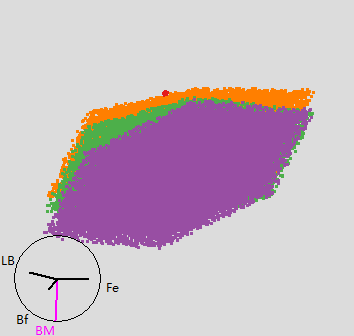
\includegraphics[width=0.25\linewidth]{Figures/QR-model-single-pixel/linear-4D-1} 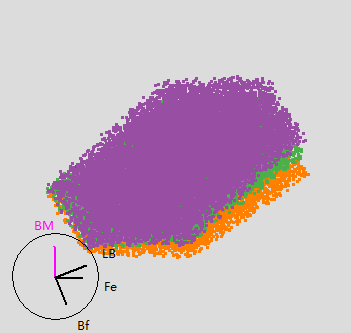
\includegraphics[width=0.25\linewidth]{Figures/QR-model-single-pixel/linear-4D-2} 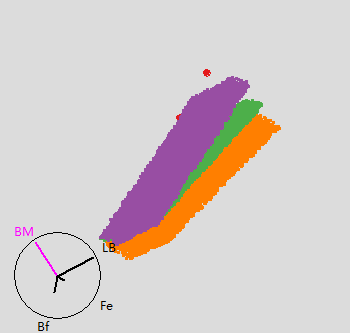
\includegraphics[width=0.25\linewidth]{Figures/QR-model-single-pixel/linear-4D-3} 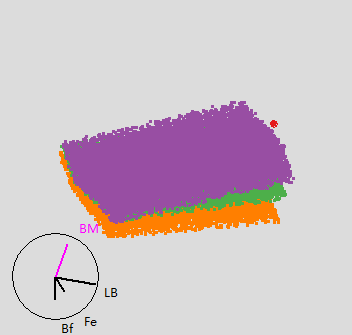
\includegraphics[width=0.25\linewidth]{Figures/QR-model-single-pixel/linear-4D-4} 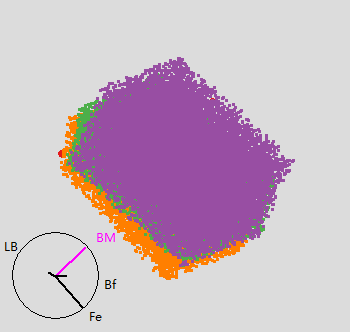
\includegraphics[width=0.25\linewidth]{Figures/QR-model-single-pixel/linear-4D-5} 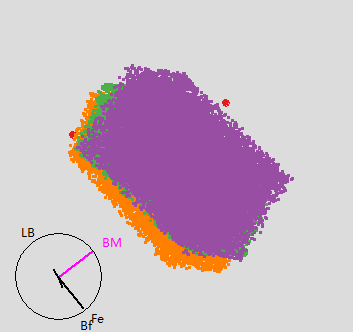
\includegraphics[width=0.25\linewidth]{Figures/QR-model-single-pixel/linear-4D-6} 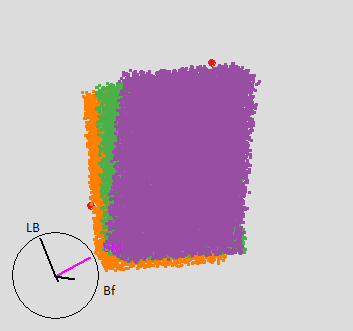
\includegraphics[width=0.25\linewidth]{Figures/QR-model-single-pixel/linear-4D-7} 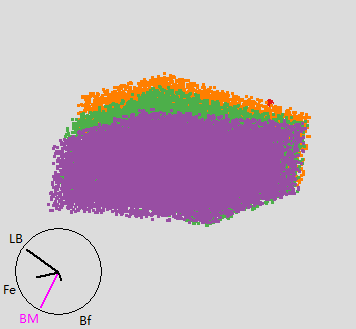
\includegraphics[width=0.25\linewidth]{Figures/QR-model-single-pixel/linear-4D-8} 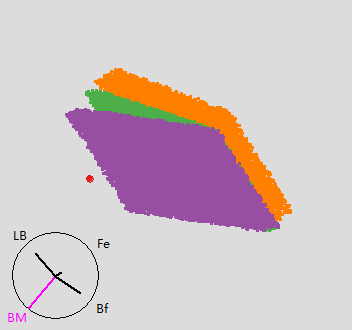
\includegraphics[width=0.25\linewidth]{Figures/QR-model-single-pixel/linear-4D-9} 

}

\caption[Linear quantile regression model with 3 response variables]{Linear quantile regression model with 3 response variables. Models on quantile 0.1, 0.5 and 0.9 corresponds to color orange, green and purple.}\label{fig:fig-name1}
\end{figure}
\end{CodeChunk}

\subsection{Non-linear Case Result}\label{non-linear-case-result}

In non-linear case, we use elliptic hyperboloid and hyperbolic
paraboloid as examples. Figure \ref{fig:fig-name2} and
\ref{fig:fig-name3} display interesting information: (a) non-linear
models show different shape on different quantiles. For the elliptic
hyperboloid, on high quantile, the non-linear model have largest
curvature comparing to models on quantile 0.5 and 0.1, while model on
quantile 0.1 has the smallest curvature. For the hyperbolic paraboloid,
the curvature of models various among quantiles much larger. (b) The
relative locations of models are maintained based on the quantile of
data. (c) no clustered or sparsed region exists in data and no
suspicious outlier exists.

\begin{CodeChunk}
\begin{figure}

{\centering 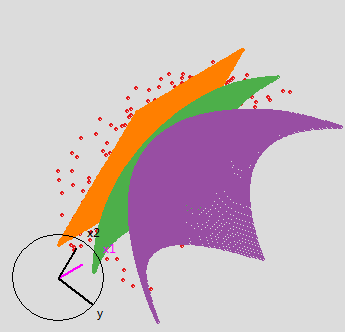
\includegraphics[width=0.26\linewidth]{Figures/QR-model/curve1-1} 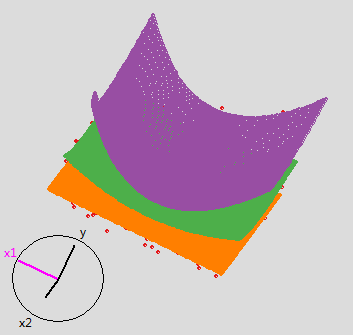
\includegraphics[width=0.26\linewidth]{Figures/QR-model/curve1-5} 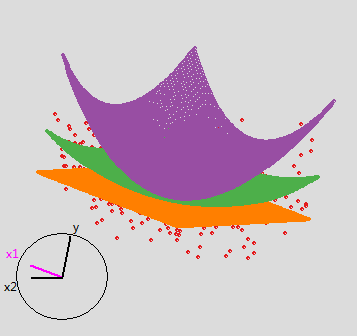
\includegraphics[width=0.26\linewidth]{Figures/QR-model/curve1-3} 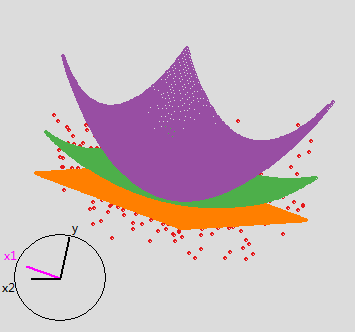
\includegraphics[width=0.26\linewidth]{Figures/QR-model/curve1-4} 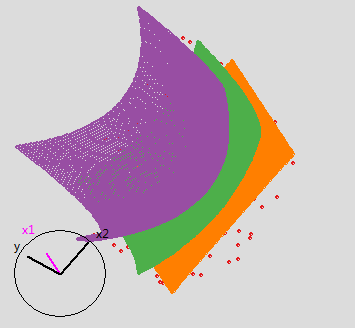
\includegraphics[width=0.26\linewidth]{Figures/QR-model/curve1-2} 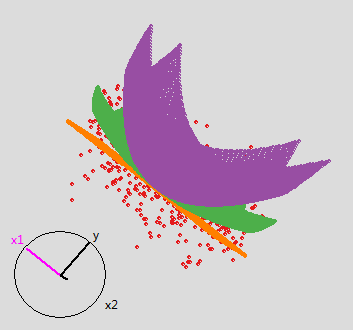
\includegraphics[width=0.26\linewidth]{Figures/QR-model/curve1-6} 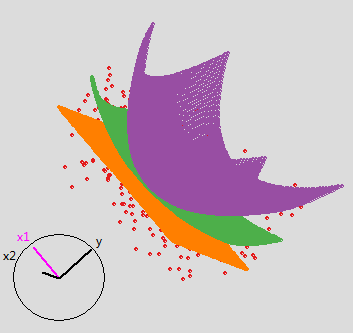
\includegraphics[width=0.26\linewidth]{Figures/QR-model/curve1-7} 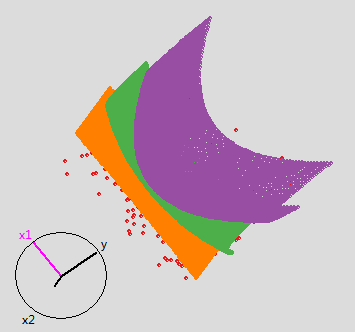
\includegraphics[width=0.26\linewidth]{Figures/QR-model/curve1-8} 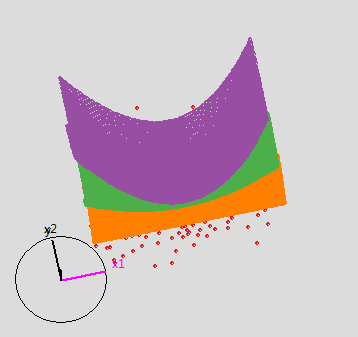
\includegraphics[width=0.26\linewidth]{Figures/QR-model/curve1-9} 

}

\caption[Non-linear quantile regression model on elliptic hyperboloid]{Non-linear quantile regression model on elliptic hyperboloid. Models on quantile 0.1, 0.5 and 0.9 corresponds to color orange, green and purple.}\label{fig:fig-name2}
\end{figure}
\end{CodeChunk}

\begin{CodeChunk}
\begin{figure}

{\centering 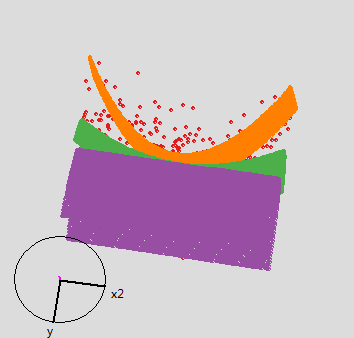
\includegraphics[width=0.25\linewidth]{Figures/QR-model/curve2-1} 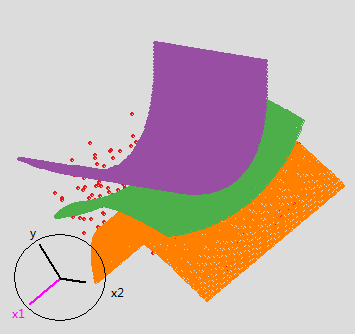
\includegraphics[width=0.25\linewidth]{Figures/QR-model/curve2-2} 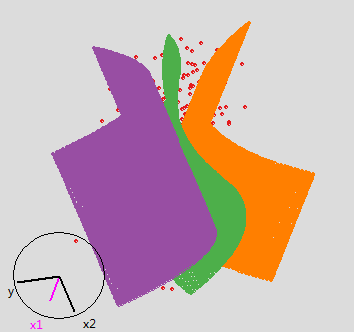
\includegraphics[width=0.25\linewidth]{Figures/QR-model/curve2-3} 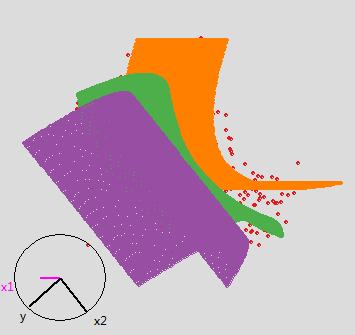
\includegraphics[width=0.25\linewidth]{Figures/QR-model/curve2-4} 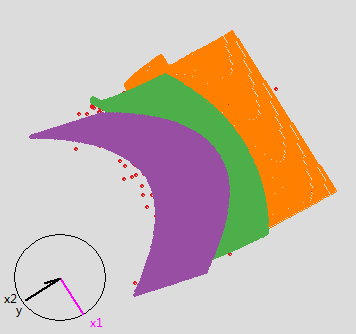
\includegraphics[width=0.25\linewidth]{Figures/QR-model/curve2-5} 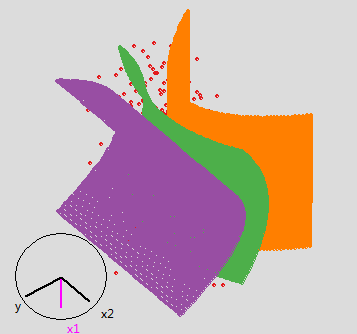
\includegraphics[width=0.25\linewidth]{Figures/QR-model/curve2-6} 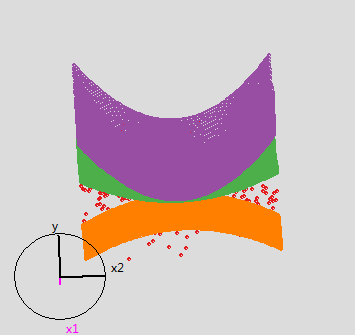
\includegraphics[width=0.25\linewidth]{Figures/QR-model/curve2-7} 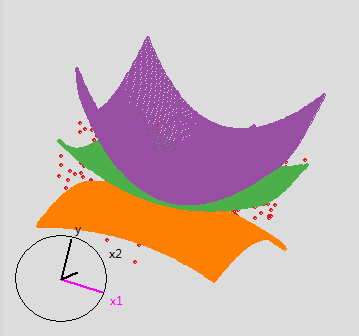
\includegraphics[width=0.25\linewidth]{Figures/QR-model/curve2-8} 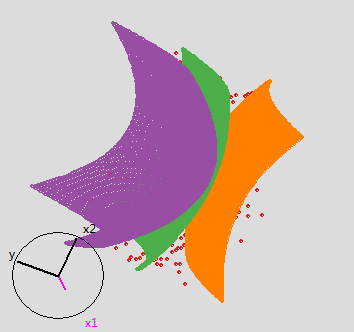
\includegraphics[width=0.25\linewidth]{Figures/QR-model/curve2-9} 

}

\caption[Non-linear quantile regression model on elliptic hyperboloid]{Non-linear quantile regression model on elliptic hyperboloid. Models on quantile 0.1, 0.5 and 0.9 corresponds to color orange, green and purple.}\label{fig:fig-name3}
\end{figure}
\end{CodeChunk}

\section{Summary and Future Work}\label{summary-and-future-work}

The first part of this paper presents R package \texttt{quokar} for
outlier diagnostic of quantile regression. The package contains methods
for outlier detecting. We considered diagnostic methods corresponding to
estimation with none error term distribution assumption, error term with
asymmetric Laplace distribution assumption and Bayesian estimating
framework. The results are provided in tidy data form which can be
directly used for plot. In addition, we provide some visualization
methods for the diagnosed results.

In data example, it was shown that \texttt{quokar} provides convenient
tools to detect suspicious outliers in quantile regression. Future
versions of the package will focus on supporting other diagnotic methods
such as methods for high dimensional data or extreme quantiles and
improving computational efficiency.

Another contribution of this paper is proposed a general framework to
visualize quantile regression in high dimensional data space. Our
visualization tool is \texttt{GGobi}. We provide integrated plot of
quantile regression models and original data. Our future work will
continue to explore visual methods for the outlier diagnostic models in
data space. We are trying to do model performance comparison with
\texttt{GGobi}.

\bibliography{reference}


\end{document}

